\documentclass{fhnwreport} %
\usepackage[ngerman]{babel}
\usepackage[T1]{fontenc}
\usepackage[utf8]{inputenc}
\usepackage{tikz}
\usepackage{amsmath}
\usetikzlibrary{arrows}
\usepackage{lmodern}      % Type1-Schriftart für nicht-englische Texte 
\usepackage{subfigure}

%%% Harvard-Style Bibliographie
%\usepackage{natbib}
%\bibliographystyle{agsm}

%%% IEEE-Style Bibliographie
\bibliographystyle{IEEEtran}

%% Und wenn die Bibliographie im Inhaltsverzeichnis sein soll:
\usepackage[nottoc]{tocbibind}


\title{%
  {\huge Das bestimmte Integral und seine Anwendungen}\\[2ex]
  {\large Semesterarbeit Einführung in die Analysis (eana)}}
\author{Florian Thiévent}

\begin{document}

% Titel
\maketitle

\vfill

% Titelbild
% (kann man natürlich auch mit Includegraphics machen)
\begin{minipage}{\textwidth}
\begin{center}
\vspace*{5ex}
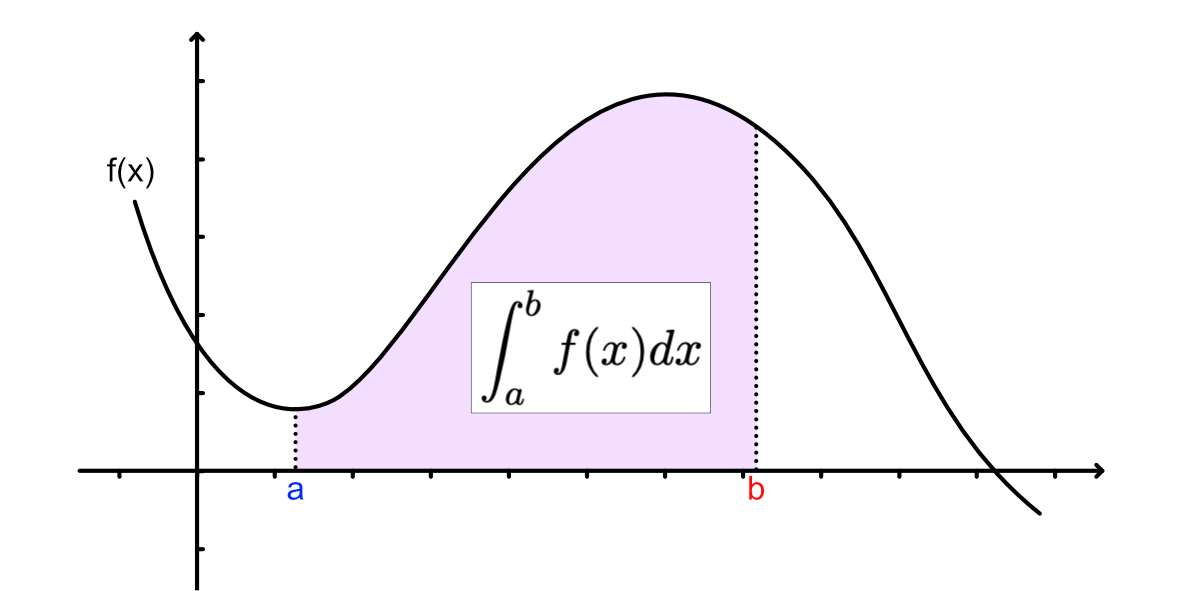
\includegraphics{titelbild}
\end{center}
\end{minipage}

\vfill

\begin{tabbing}
Dozent: \hspace{2em} \= Andreas Leiser \\[2ex]
Studiengang: \> Informatik
\end{tabbing}


\hbox{}

\clearpage

% Inhaltsverzeichnis
\tableofcontents
\clearpage

%\cite{Bosch2010}}
\section{Motivierung}
Die Integralrechnung stellt die Umkehrung der Differentialrechnung dar \cite{Bosch2010}. Dabei wird zwischen dem unbestimmten und dem bestimmten Integral unterschieden. Im unterschied zum unbestimmten Integral kann mit dem bestimmten Integral einen konkreten Zahlenwert berechnen oder das bestimmte Integral einer Funktion weisst der Funktion eine Zahl zu. Ob es sich um ein unbestimmtes oder bestimmtes Integral handelt wird durch das Vorhandensein von Integrationsgrenzen bestimmt. Das bestimmte Integral kann dazu verwendet werden den Flächeninhalt zwischen einem Graphen und der Koordinatenachse oder zwischen zwei Graphen zu berechnen. In dieser Arbeit wird das Riemann'sche Integral (auch Darboux Integral) verwendet um das bestimmte Integral zu berechnen.

\clearpage
% Abschnitt fertig

\section{Theorie: Das bestimmte Integral}
\subsection{Allgemeines}
Mit dem bestimmten Integral kann der Flächeninhalt unter einer Funktion $f$ über einem bestimmten Intervall auf der $x$-Achse berechnet werden. Man erhält für nichtnegative Funktionen bei Kurven oberhalb der $x$-Achse den positiven Flächeninhalt und bei Kurven unterhalb der $x$-Achse den negativen Flächeninhalt. 
\begin{figure*}[!h]
    \subfigure{ 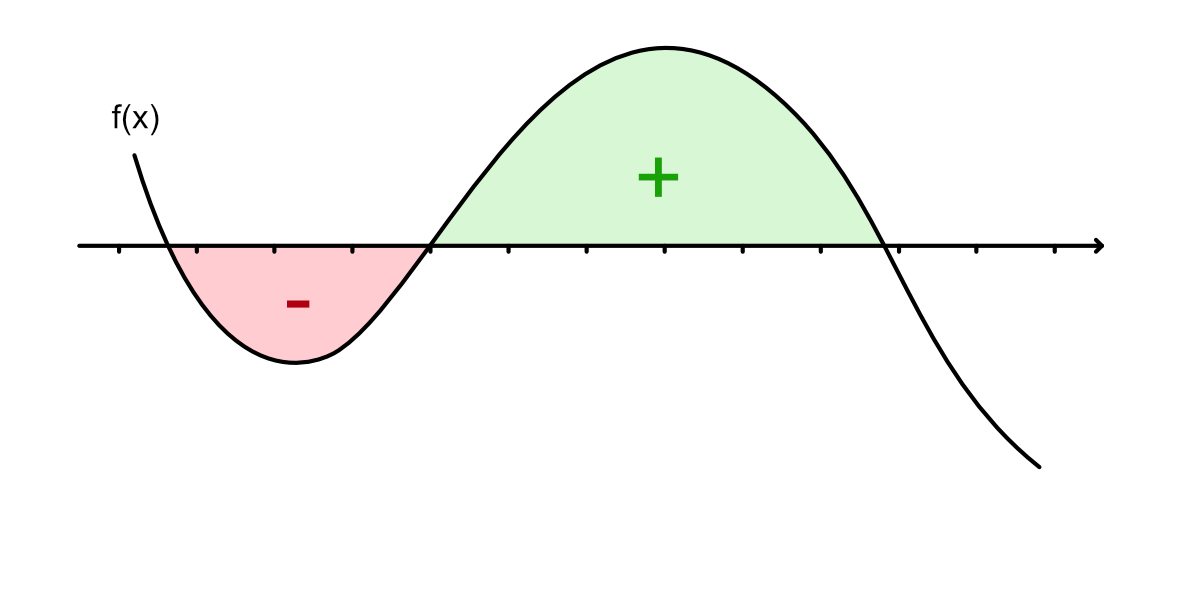
\includegraphics[width=0.49\textwidth]{orientierte-flaeche}}
    \subfigure{ 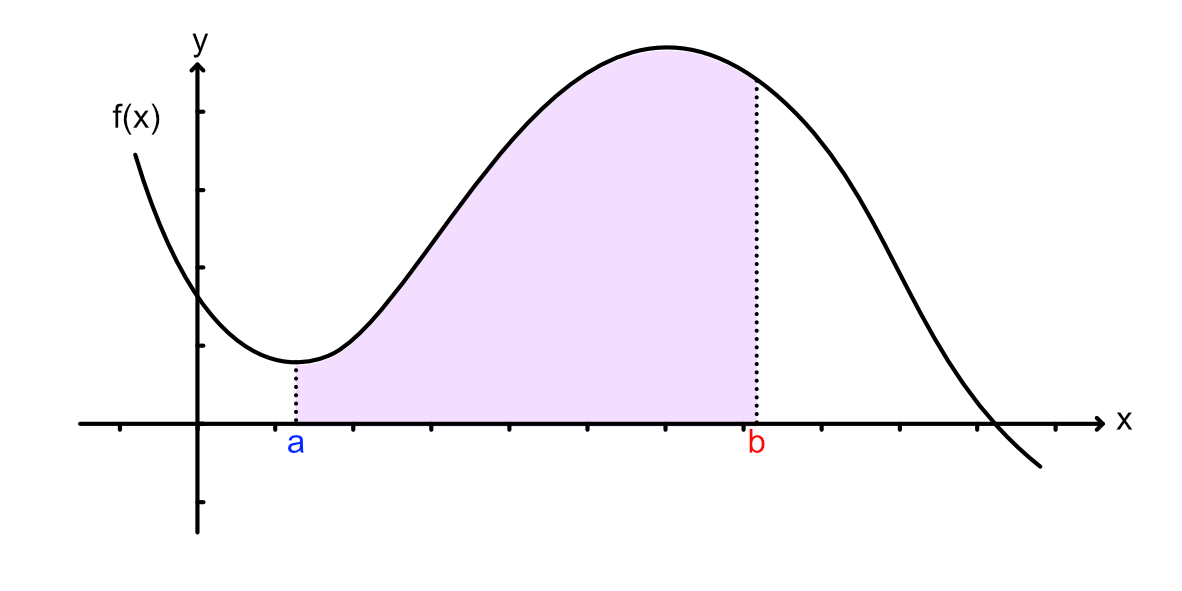
\includegraphics[width=0.49\textwidth]{flaecheninhalt}}
\caption{Orientierte Fläche (links), zu berechnender Flächeninhalt (rechts)}
\end{figure*}


\subsubsection{Vorgehen nach Riemann \cite{Riemann2020}}
Das Problem bei der Berechnung von Flächeninhalten unter einem Graphen ist, dass es keine "Formel" gibt wie man diese aus der Geometrie kennt um beispielsweise Flächen von Rechtecken, Dreiecken und Quadraten zu berechnen. Es ist jedoch möglich, dieses Wissen zu nutzen um eine Näherung zu erhalten. Die Fläche zu berechnende Fläche des Intervalls wird durch die Fläche eines Rechtecks ersetzt.	
\begin{figure*}[!h]
\centering
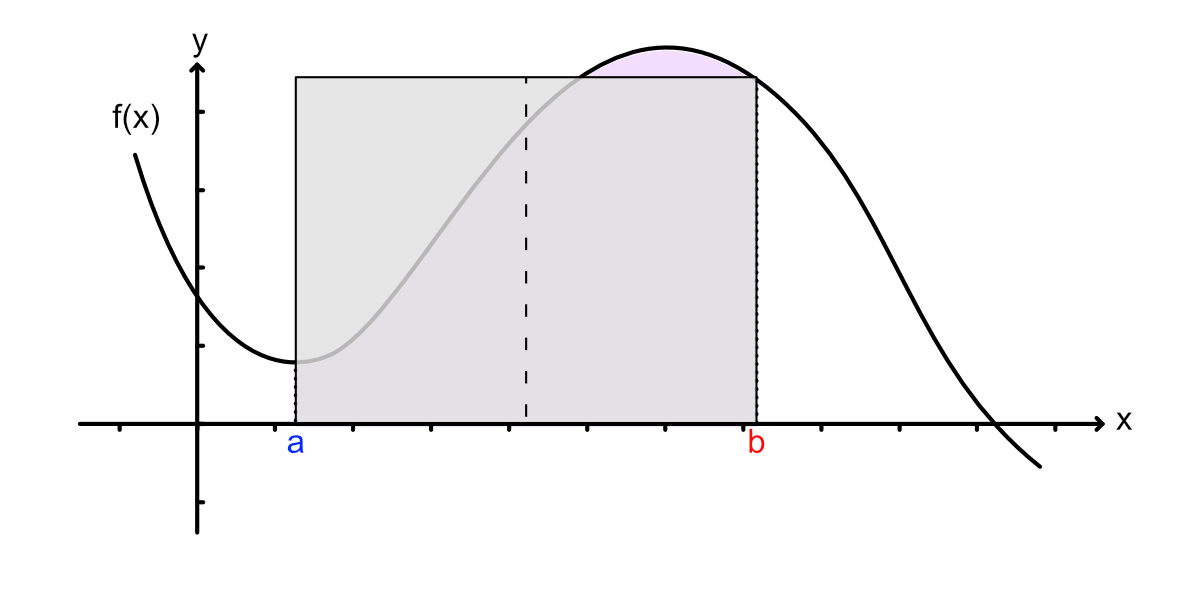
\includegraphics{grobe-approximierung-riemann.png}
\caption{Grobe Approximierung}
\label{Grobe Approximierung}
\end{figure*}

Dies Annäherung ist jedoch noch viel zu grob. Durch das Unterteilen des grossen Rechteckes in viele kleine, kann eine viel bessere Approximation erreicht werden. Wir zerlegen somit das Intervall $I := [a,b]$ in mehrere gleich grosse Teile. Werden nun diese Intervalle immer kleiner gemacht, dann wird die Summe der Flächen der Rechtecke immer mehr an die Fläche zwischen dem Graphen und der $x$-Achse angenähert.

\begin{figure*}[!h]
    \subfigure{ 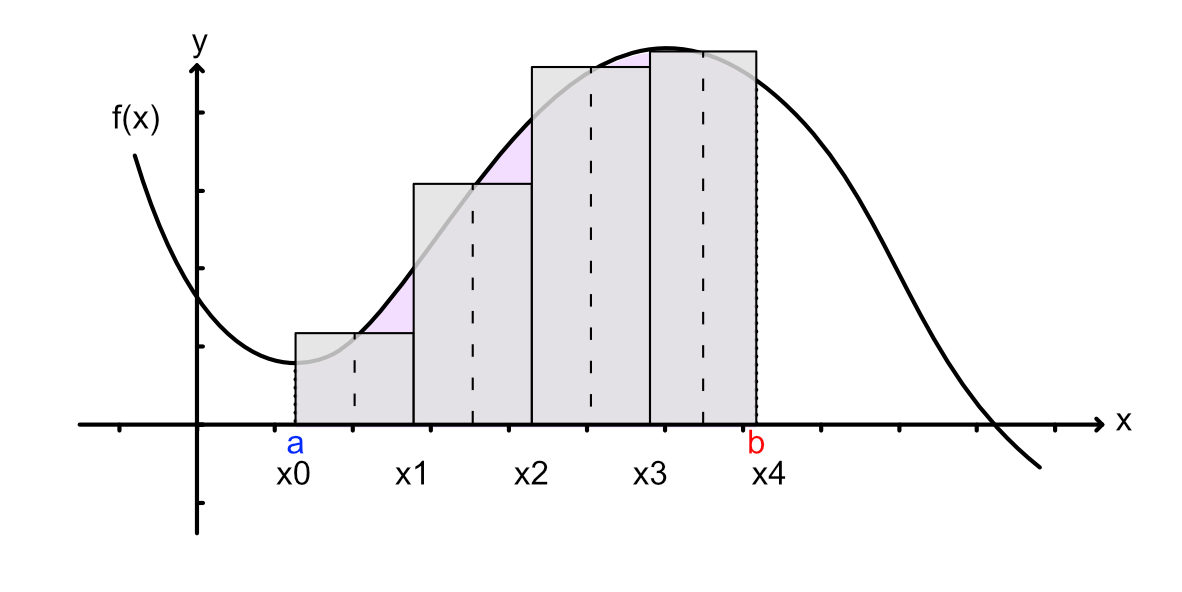
\includegraphics[width=0.49\textwidth]{mittlere-approximierung-riemann}}
    \subfigure{ 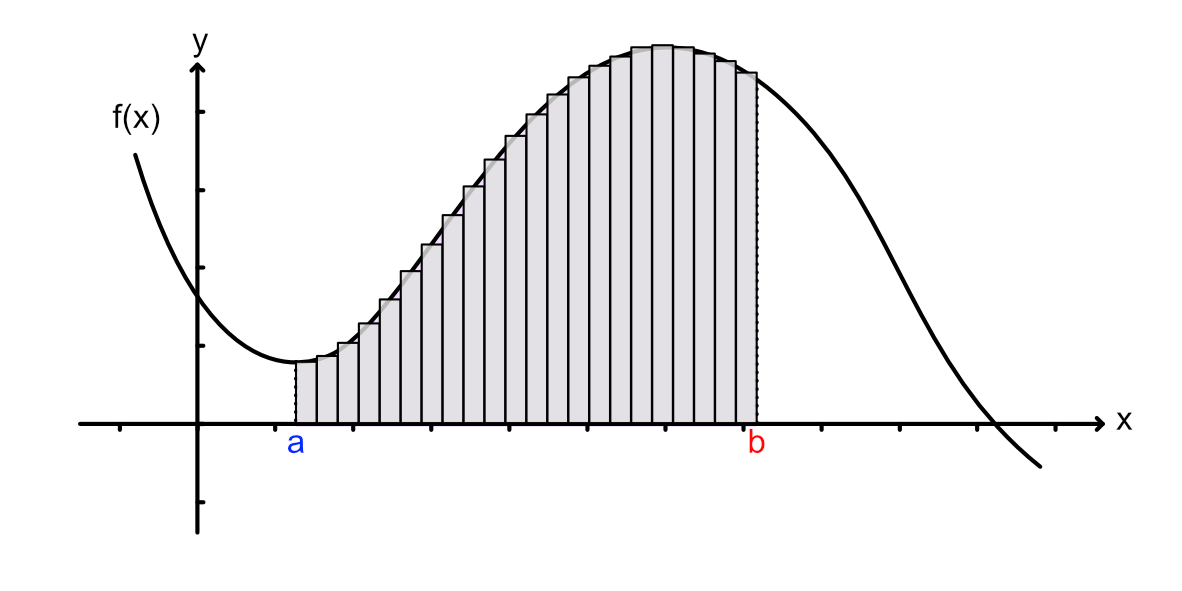
\includegraphics[width=0.49\textwidth]{feine-approximierung-riemann}}
\caption{Mittlere- (links) und feine Approximierung (rechts)}
\label{Mittlere- (links) und feine Approximierung (rechts)}
\end{figure*}


%ACHTUNG EVENTUELL ENTFERNEN DES PAGEBREAK NÖTIG
\pagebreak

Zählt man die Flächen der Rechtecke der mittleren Approximation aus \ref{Mittlere- (links) und feine Approximierung (rechts)} zusammen, erhält man eine erste Idee des Flächeninhaltes unter dem Graphen. Wir müssen also 
\[
	F = f(x)*(x_1-x_0)+f(x)*(x_2-x_1)+f(x)*(x_3-x_2)+f(x)*(x_4-x_3)
\]

rechnen. Zur übersichtlichkeit fassen wir dies zusammen:
\[
	S_3 = \sum_{i=1}^{3} f(x_i)\underbrace{(x_i-x_{i-1})}_{\substack \Delta x_i}
\]

Da dies immernoch zu wenig genau ist, brauchen wir nicht 4 Rechtecke sondern $n$. Schreiben wir die Summe als allgemeiner

\[
	S_n = \sum_{i=1}^{n} f(x_n)\Delta x_i
\]

Diese allgemeine Form nennt man auch eine Riemann Summe. Um nun den korrekten Wert für die Fläche unter dem Graphen zu erhalten reicht eine Summe mit $n$ wiederholungen nicht aus, wir benötigen unendlich viele

\[
	\lim_{x\to\infty} S_n = \int_{x_0}^{x_n} f(x) dx
\]

Das so gefundene Integral nennt man das Riemann Integral. $f(x)$ ist dabei die Höhe des erzeugten (unglaublich) schmalen Rechtecks, $dx$ die Breite des Rechtecks.

\subsubsection{Vorgehen nach Darboux \cite{Darboux2020}}
Eine weitere Methode stellt die Darboux Methode dar. Diese ist nach dem französischen Mathematiker Gaston Darboux \cite{Darboux2020} benannt.


Da dies keine gute Annäherung ist, wird das einzelne Rechteck in viele kleinere Rechtecke aufgeteilt und so besser approximiert. Der Grenzwert liefert schliesslich den exakten Wert. Die Rechtecke werden in zwei Kategorien eingeteilt. Rechtecke unter der Kurve bilden die Untersumme, Rechtecke oberhalb der Kurve bilden die Obersumme. Das Verfahren mit Unter- und Obersumme wurde durch den französischen Mathematiker Gaston Darboux hergeführt und lieferte damit eine neue Sichtweise auf das Riemann-Integral \cite{Darboux2020}.

\begin{figure*}[!h]
    \subfigure{ 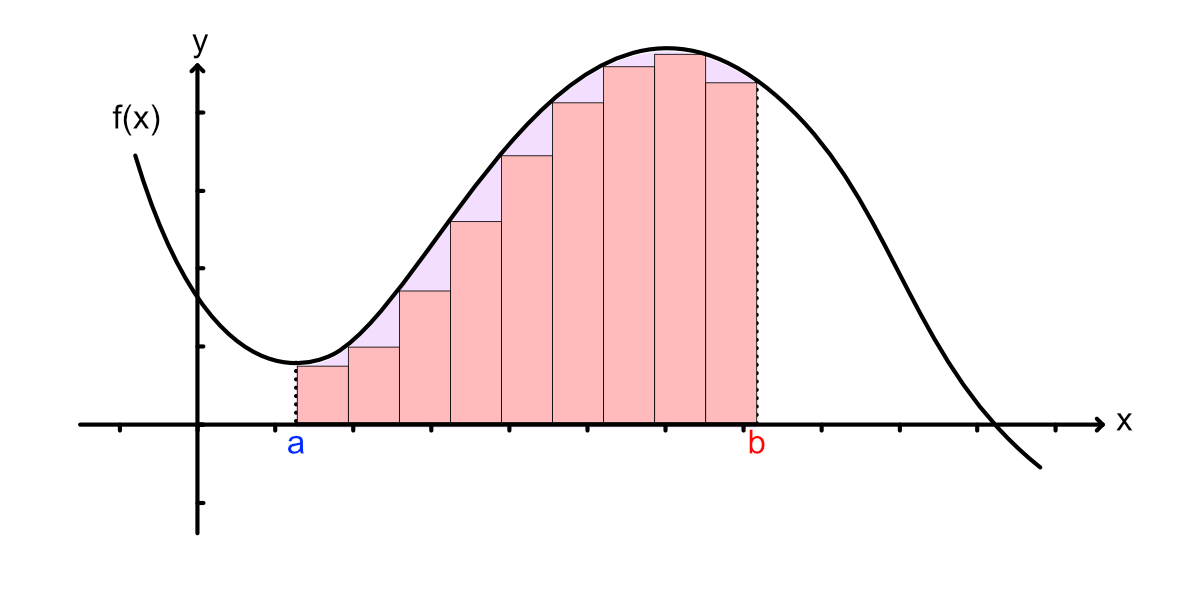
\includegraphics[width=0.49\textwidth]{untersumme}}
    \subfigure{ 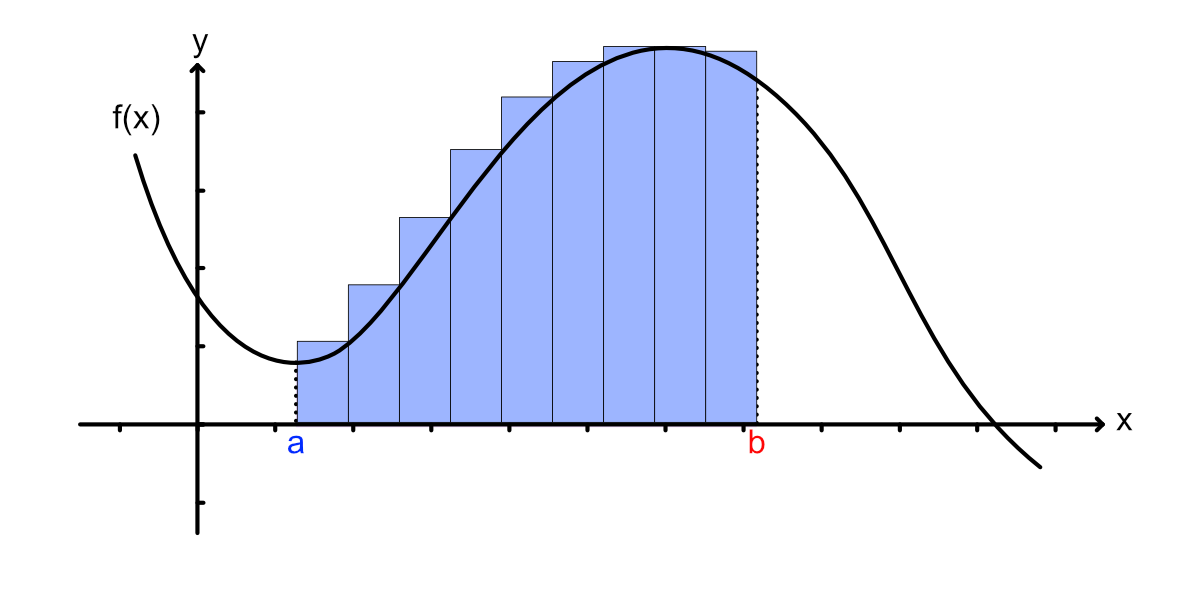
\includegraphics[width=0.49\textwidth]{obersumme}}
\caption{Unter- und Obersumme}
\end{figure*}

\subsection{Definition des bestimmten Integral}
\subsection{Rechenregeln für bestimmte Integrale}



\clearpage
% Abschnitt fertig

\section{Beispiele und Anwendungen}
\subsection{Rechenbeispiele}

Ein erstes einfaches Beispiel. Zu berechnen ist das Integral der Funktion $f$(x)=2x im Intervall [\color{blue}1\color{black};\color{red}3\color{black}].

\[
\int_{\color{blue}1}^{\color{red}3} \! 2x \, \mathrm{d}x = \left[x^2\right]_{\color{blue}1}^{\color{red}3} = {\color{red}3}^2 - {\color{blue}1}^2 = 8
\]
  
\begin{figure*}[!h]
    \subfigure{ 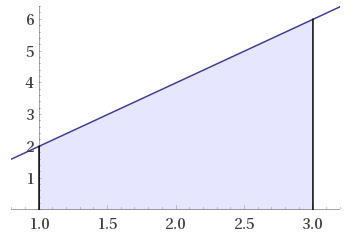
\includegraphics[width=0.49\textwidth]{ex1_integral}}
    \subfigure{ 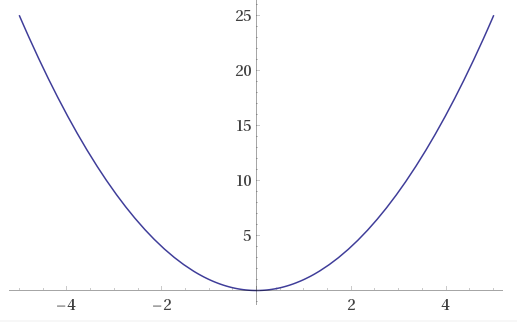
\includegraphics[width=0.49\textwidth]{ex1_stammfunktion}}
\caption{Plot zu Integral- und Stammfunktion Beispiel 1}
\end{figure*}

\subsection{Integrieren mit Python}


\clearpage
% Abschnitt fertig

\bibliography{example,IEEEabrv}

\end{document}

